\section{Robinhood Dataset}
\subsection{Description of the Dataset}
This data is retrieved from \url{https://robintrack.net/}, the creator retrieved data from the official Robinhood API.

The dataset contains the number of Robinhood users holding at least one share of 8,221 securities. The available data spans from February 5, 2018, to August 13, 2020, covering 818 days (data is available also for non-trading days). Although the data was originally recorded hourly, I aggregated it to a daily frequency by computing the average number of holders per day to simplify computations due to the dataset's size. This aggregation can be easily reversed if needed. 


\begin{figure}[h!]
        \centering
        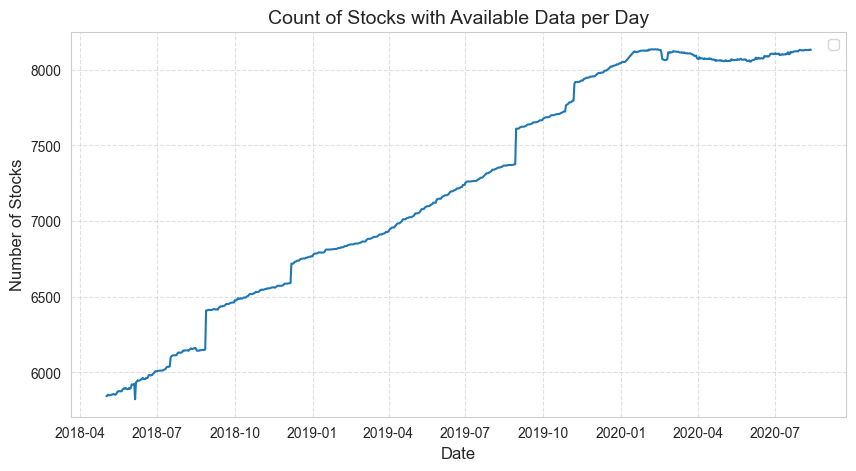
\includegraphics[width=0.8\linewidth]{../images/no_stocks_date.png}
        
\end{figure}


\paragraph{Handling NaNs}  
The original dataset contains missing values for 3,331 securities, primarily in the earlier periods. In some cases, assets appear in the dataset only after a certain date, despite being publicly traded before. It is important to distinguish between missing values and zero values, as they represent different concepts. Some securities exhibit a sudden increase from zero to a larger number of holders, but interpreting these as errors would impose an assumption on investor behavior.  

\noindent Additionally, 1,248 securities have at least one recorded zero in the number of holders. The majority of missing data corresponds to small-cap stocks, which collectively account for at most 3 percent of total market capitalization. Given the limited impact of these securities on overall retail activity, I opted to remove all securities with missing values to ensure consistency in the dataset.  



\subsubsection{Distribution of Key Features (Log-Transformed)}
The distributions of trading volume, market capitalization, and retail holders were initially highly skewed, with a few extreme values dominating the dataset. To address this, I applied a logarithmic transformation: $x^\prime = \log(1+x)$. 

This transformation reduces the impact of outliers, enhances interpretability by making the data more symmetric, and facilitates comparisons between stocks of different sizes.

The key observations after applying the transformation are:
\begin{itemize}
    \item \textbf{Trading Volume:} The distribution appears approximately normal, centered around a peak, with a slight left tail. While most stocks have relatively low trading volume, a few highly traded stocks, such as large-cap or meme stocks, exist but no longer dominate the distribution.
    \item \textbf{Market Capitalization:} The transformed market capitalization data exhibits a bell-shaped curve, suggesting a more balanced spread across small, mid, and large-cap stocks. However, some large-cap stocks remain in the extreme right tail, indicating that a few companies, such as Apple and Microsoft, are significantly larger than the majority.
    
    \item \textbf{Retail Holders:} The number of retail holders follows a roughly log-normal distribution, confirming that a small number of stocks attract massive retail participation while most remain relatively unpopular. The left tail suggests that many stocks have very few retail holders, reinforcing the notion that retail trading is concentrated in a subset of securities.
\end{itemize}

\begin{figure}[h!]
    \centering
    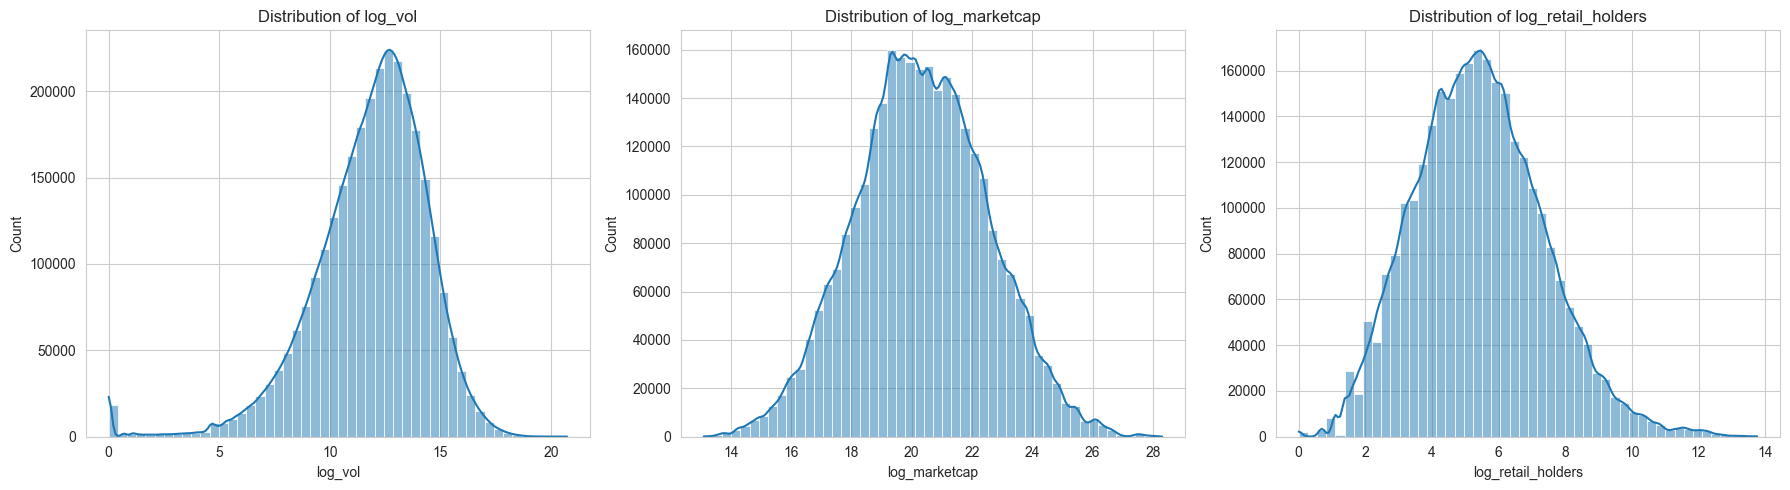
\includegraphics[width=1\linewidth]{../images/Distributions.png}
\end{figure}












\subsection{Comparing the Portfolios}
\subsubsection{Methodology and Overview} 
To build a representative portfolio of the average Robinhood investor, it is necessary to retrieve the prices of the securities. A capitalization-weighted approach can be used, multiplying the price of each security by the number of users who hold it. This approach assumes that all Robinhood users hold a similar number of shares for a given ticker, or that the distribution of shares held per user follows a normal distribution.  

Over the years covered in the dataset, Robinhood has gained a significant number of users. Data on active users is available on Statista\footnote{\url{https://www.statista.com/statistics/822176/number-of-users-robinhood/}}, though only on a yearly basis. Comparing the Statista figures with Robinhood's reported numbers for 2023 suggests that the active user count corresponds to December 31 of each year. This data could later be used to normalize the number of users and build a reference portfolio.  

The total number of open positions can be computed as the sum of all investors who hold at least one security in each asset, effectively a row-wise sum of the dataset.  

Market data for all securities was retrieved from the CRSP\footnote{The Center for Research in Security Prices, based at the University of Chicago, provides high-quality historical market data widely used in finance research and investment analysis.} database, accessed via WRDS. However, only 8,099 securities are available in CRSP, as it focuses exclusively on American assets. The difference in open positions between the full dataset and the CRSP subset is minimal. If, instead, all securities with missing values are dropped, leaving only 5,221 securities, the gap widens.

\begin{figure}[h!]
        \centering
        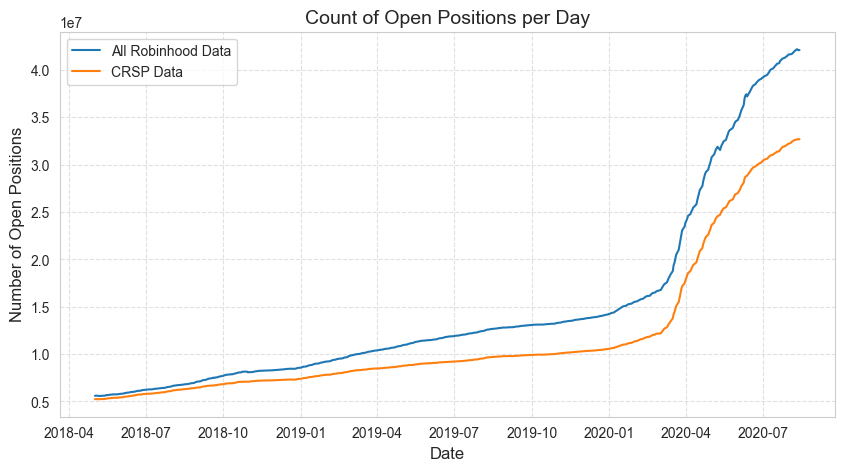
\includegraphics[width=0.8\linewidth]{../images/no_positions_vs_date_drop.png}
\end{figure}

The graph illustrates the  count of open positions per day  on Robinhood from April 2018 to mid-2020, showing a  steady increase  over time, with a  sharp acceleration in early 2020. This surge aligns with the onset of the  COVID-19 pandemic, which likely drove a significant influx of new retail investors seeking market opportunities amid economic uncertainty and stimulus checks. 



\subsubsection{Retail Investors Prefer "Famous" Stocks}

The majority of the securities are common shares, representing about 57.9\%. ETFs represent about 23.7\% and other funds are the 9.2\% of the dataset. Other structured investments, REITs, and ADRs cover the remaining part.

Analysing the securities by market capitalisation about 82.9\% is represented by stocks and 9.6\% by ETFs. If we look at the "Retail Market Cap" (i.e. number of positions times price), 89.2\% of securities are stocks and 5.8\% are ETFs.  

Looking at the securities Robinhood users prefer holding, ranked by "Retail Market Cap", investors prefer holding smaller cap stock. A qualitative analysis shows "famous" stocks, such as Tesla, Starbucks, and Nvidia to name a few, to appear among the most popularly owned.

\subsubsection{Possible Measures of Divergence} 
\paragraph{Rank Distance} 
To describe the preference of retail investors for smaller cap stock I propose the following measure:
\begin{align*}
    d_R = \sum_{i=1}^N \frac{R^{\text{Mkt}}_i-R^{\text{RH}}_i}{R^{\text{RH}}_i}
\end{align*}
Where $R^{\text{Mkt}}_i$ is the rank of the $i^\text{th}$ security by market cap, and $R^{\text{RH}}_i$ is the rank by retail market cap. The normalization by $R^{\text{RH}}_i$ reduces the impact of small-cap stocks with minor ranking differences.

\begin{figure}[h]
        \centering
        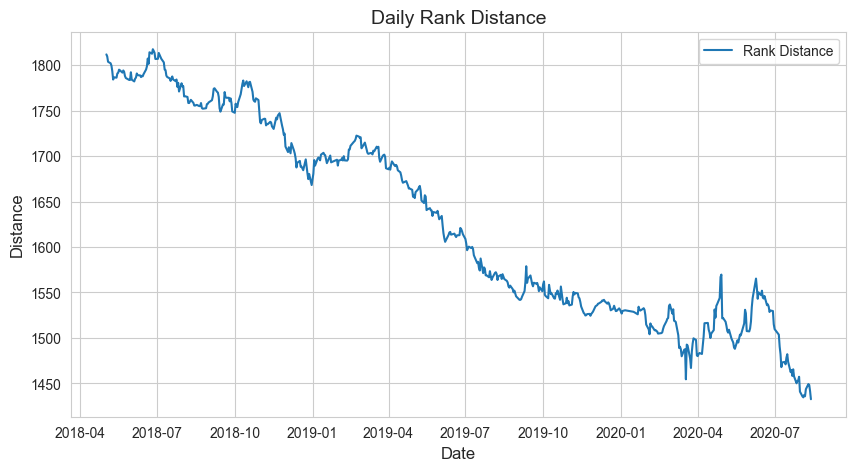
\includegraphics[width=0.8\linewidth]{../images/rank_distance.png}
\end{figure}

The plotted Daily Rank Distance suggests a clear downward trend from early 2018 to mid-2020, indicating that the ranking of stocks by retail market cap has become increasingly aligned with the ranking by total market cap. Initially, the distance is above 1800, gradually declining towards 1450. This implies that retail investors, who originally exhibited a stronger preference for smaller-cap stocks, have progressively shifted towards stocks that are more representative of the broader market.

Between 2018 and 2019, the decline is relatively steady, reflecting a gradual change in retail investment behavior. However, the trend accelerates in 2019 and 2020, suggesting a more pronounced shift. The beginning of 2020 shows increased volatility, with occasional upward spikes, which could be attributed to market disruptions, possibly linked to the COVID-19 crash and the subsequent retail trading boom. The rapid expansion of retail investing during this period, fueled by stimulus checks and zero-commission trading, may have led to temporary deviations, but the overall trend continues downward.

A sustained decrease in rank distance suggests that retail investors have moved closer to institutional preferences, potentially increasing their exposure to large-cap stocks or index-tracking assets. If this trend persists, it would indicate a continued assimilation of retail behavior into the broader market structure. Conversely, a reversal in this pattern could signal renewed speculative activity or a shift back to small-cap stocks.
